\chapter{Implementácia}
\label{kapitola5}
Táto kapitola popisuje čitateľovi samotnú implementáciu aplikácie. Čitateľ sa oboznámi s použitými nástrojmi pri tvorení aplikácie a s postupom implementácie frontendovej a backendovej časti. Prvým bodom implementácie bolo vytvorenie zložky mono-repozitára zahrňujúci obe časti aplikácie.

\section{Git a GitHub}
\label{git}
Pred začatím písania zdrojového kódu sa najprv spojazdnil verzovací systém Git cez GitHub. Cieľom bolo verzovanie samotného zdrojového kódu aj dokumentácie. Pre jednoduchšiu orientáciu v repozitároch sa vytvorila GitHub organizácia, ktorá obsahuje monorepozitár pre zdrojový kód a repozitár pre dokumentáciu na jednom mieste. Monorepozitár je repozitár obsahujúci viacero projektov, v tomto prípade projekt klienta a servera. Organizácia aj repozitáre sú verejne dostupné pod odkazom:
    \begin{verbatim}
        https://github.com/AdamAbrahaamBC
    \end{verbatim}

GitHub ponúka projektom organizačnú tabuľku(project board). Tabuľka pomáha v organizovaní úloh a poskytuje jednoduchší prehľad projektu. Môže mať ľubovolný počet kolóniek, do ktorých sa prideľujú jednotlivé úlohy. V tomto projekte bolo postačujúce vytvorenie troch kolóniek. Kolónka \texttt{To Do} obsahuje ešte nezačaté úlohy, kolónka \texttt{In progress} úlohy, ktoré sa práve riešia a kolónka \texttt{Done} už dokončené a zatvorené úlohy. Pri vytvorení novej úlohy sa úloha automaticky priradí do kolónky \texttt{To Do}. Pri zvolení následujúcej úlohy musí byť manuálne premiestnená do kolónky \texttt{In Progress} a pri jej zatvorení sa automaticky premiestni do kolónky \texttt{Done}.


K jednotlivým úlohám sú pridelené štítky. Štítky označujú o aký typ úlohy sa jedná. Dostupné štítky projektu sú nasledujúce.

    \begin{itemize}
        \item\textbf{backend} - označuje úlohy týkajúce sa backendu
        \item\textbf{frontend} - označuje úlohy týkajúce sa frontendu
        \item\textbf{db} - označuje úlohy na databáze
        \item\textbf{bug} - označuje úlohy obsahujúce chybu v aplikácii
        \item\textbf{todo} - označuje zatiaľ nezačaté úlohy
        \item\textbf{done} - označuje dokončené úlohy
    \end{itemize}
    
    \begin{figure}[!hbt]
        \centering
        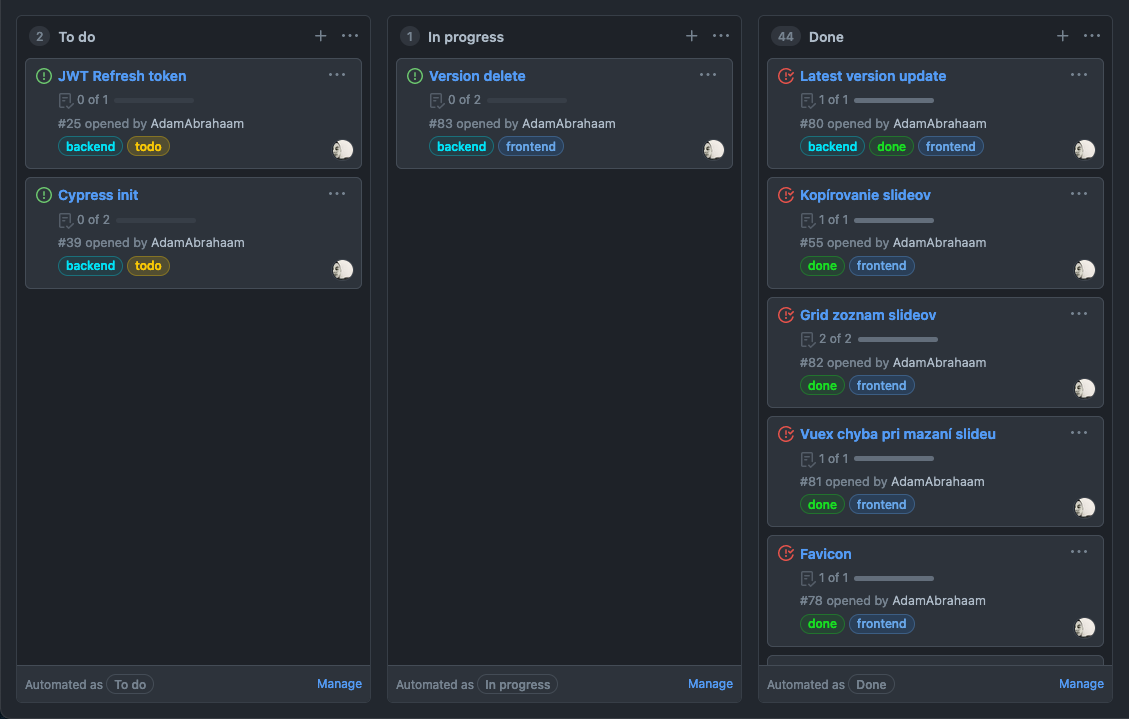
\includegraphics[scale=0.3]{obrazky/board.png}
        \caption{Organizačná tabuľka projektu}
        \label{pic:board}
    \end{figure}

\section{Implementácia frontendu}
\label{impfrontend}
Implementácia frontendu sa začala stiahnutím \texttt{Node.js}. Node.js obsahuje nástroj \texttt{npx} pre spúšťanie balíčkov. Pomocou npx sa vytvoril Nuxt.js projekt cez terminálový príkaz: \texttt{npx create-nuxt-app <názov-projektu>}. 

\vspace{5mm}
Po zadaní príkazu sa spustí sprievodca inštalácie, kde sa zvolil:
    \begin{itemize}
        \item správca balíčkov \texttt{npm}
        \item podpora pre \texttt{TypeScript}
        \item \texttt{Buefy} framework pre užívateľské prostredie
        \item komunikačný modul \texttt{axios}
        \item analyzačný nástroj zdrojového kódu \texttt{ESLint} 
        \item \texttt{jednostránkový} typ aplikácie(SPA)
    \end{itemize}
    
\vspace{5mm}
Balík Composition API je potrebné nainštalovať cez npm pomocou príkazu \texttt{npm install @nuxtjs/composition-api --save} a treba ho pridať medzi Nuxtom používané moduly v súbore \texttt{nuxt.config.js}.

Súbor \texttt{nuxt.config.ts} treba hneď na začiatku zvýrazniť. Je to súbor obsahujúci konfigurácie aplikácie. Nastavujú sa v ňom vlastnosti hlavičky aplikácie, ako názov, meta značky a ikonka. Obsahuje nastavenia smerovania, TypeScriptu, autentifikačného modulu, globálnych CSS súborov a ostatných rozširovacích modulov.

Nuxt.js udáva jednoduchý štartovací bod pre vývoj aplikácie. Po inicializácii projektu skonštruuje štruktúru aplikácie, ktorá je doplnená adresármi \texttt{composable} a \texttt{models}. štruktúru aplikácie dokopy tvoria nasledujúce adresáre:

\vspace{5mm}
\dirtree{%
.1 /client.
.2 /\.nuxt.
.2 /assets.
.2 /components.
.2 /composable.
.2 /dist.
.2 /layouts.
.2 /models.
.2 /node\_modules.
.2 /pages.
.2 /plugins.
.2 /store.
}
\vspace{5mm}

\subsection*{Mobilná verzia}
Aplikácie je určená hlavne pre webové prehliadače. Mobilná verzia je kompaktnejšia. Neobsahuje funkcionalitu vytvárania a upravovania prezentácií. Zobrazovanie a funkcie pre správu prezentácií sú avšak naďalej dostupné. Pohľad domovskej stránky a detailu prezentácie v mobilnej verzii je zobrazený na obrázku \ref{pic:domovska_stranka} a \ref{pic:mobil_detail}

\begin{figure}[!hbt]
\centering
\begin{minipage}{.5\textwidth}
  \centering
  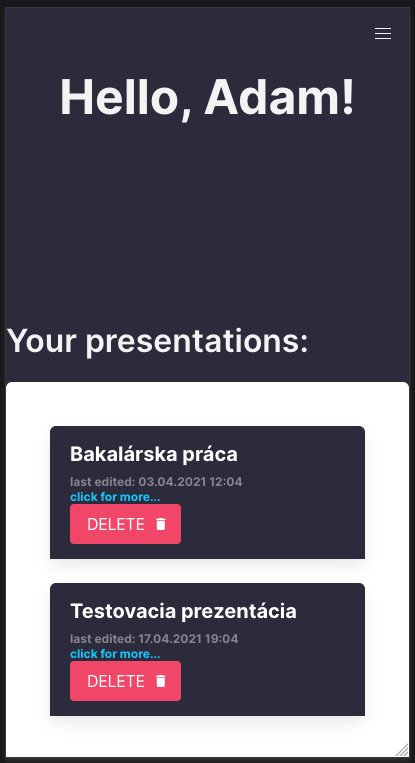
\includegraphics[scale=0.2]{obrazky/mobil_domovska_stranka.png}
  \caption{Mobilná verzia domovskej stránky}
  \label{pic:mobil_domovska_stranka}
\end{minipage}%
\begin{minipage}{.5\textwidth}
  \centering
  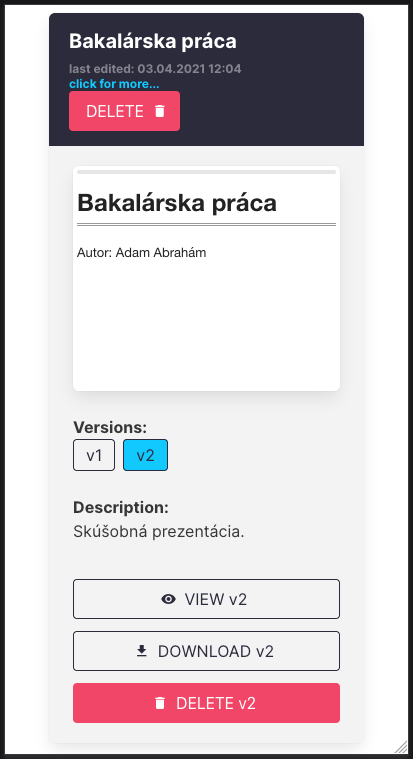
\includegraphics[scale=0.2]{obrazky/mobil_detail.png}
  \caption{Mobilná verzie detailu prezentácie}
  \label{pic:mobil_detail}
\end{minipage}
\end{figure}

\subsection{Autentifikácia užívateľov}
\label{auth}
Autentifikáciu užívateľov má na starosti autentifikačný nuxt modul. Modul sa nainštaluje cez npm, príkazom \texttt{npm install --save-exact @nuxtjs/auth-next} a pridal do nuxt konfiguračného súboru medzi moduly. Autentifikačný modul vyžaduje inštaláciu nuxt modulu \texttt{axios} pre HTTP komunikáciu. 

Middleware je globálne nastavený v nuxt konfiguračnom súbore na každú jednu trasu aplikácie okrem stránky prihlasovania, registrovania a zobrazenia prezentácie v prezentačnom móde. Na týchto stránkach je middleware manuálne vypnutý a sú dostupné bez autentifikácie. Neprihlásený užívateľ pri navštívení stránky, ktorá autentifikáciu vyžaduje je automaticky presmerovaný na prihlasovaciu stránku.

Modul funguje na báze schém. Schémy definujú logiku autentifikácie. Projekt môže obsahovať viacero schém pre rôzne typy prihlasovania, napríklad cez Facebook, Google, atď. V aplikácii je implementovaná lokálna schéma na báze JWT tokenov. Jej konfigurácia sa nachádza v konfiguračnom súbore. 

Modul poskytuje aplikačné rozhranie cez kľúčové slovo \$auth, ktoré je globálne dostupné cez kontext aplikácie. Prihlasuje sa cez funkciu \texttt{\$auth.loginWith('local', { data: PRIHLASOVACIE\_ÚDAJE })}. Modul pošle na prihlasovací koncový bod prihlasovacie údaje. Pri úspešnom prihlásení API vráti v HTTP odpovedi autentifikačný token užívateľa, ktorý sa uloží do koláčov(cookies) aplikácie a modul si automaticky vypýta údaje o užívateľovi podľa tokenu. Údaje užívateľa sú dostupné cez objekt \texttt{\$auth.user}. Odhlasuje sa cez \texttt{\$auth.logout()}.

\subsection{Smerovanie a stránky}
Smerovanie vo Vue.js sa rieši cez balík \texttt{vue-router}. Jednotlivé vlastnosti trias ako URI, komponenta pre vykreslenie a  potomky je potrebné nakonfigurovať v konfiguračnom súbora. 

Nuxt.js uľahčuje vývoj aj v tomto smere. Pomocou frameworku nie je potrebné konfigurovať trasy, Nuxt.js zoberie všetky zložky a súbory z adresára \texttt{pages} a skonštruuje smerovanie aplikácie automaticky. Každá zložka v adresári je samostatná trasa, ktorá obsahuje súbor \texttt{index.js} zahrňujúca komponentu stránky. Každá komponenta stránky je samostatná Vue.js komponenta so špeciálnymi atribútmi a funkciami. Zložky môžu obsahovať ďalšie vnorené zložky pre vnorené trasy. Zložky pomenované s podčiarkovníkom(\_) na začiatku sú dynamické, ich hodnota sa mení. Dynamické stránky v aplikácii sa využívajú pre konkrétnu prezentáciu \texttt{/presentation/\_id} a pre konkrétnu verziu prezentácie \texttt{/presentation/\_id/\_version}, kde sa tieto názvy menia podľa potreby. Obsah adresára:

\vspace{5mm}
\dirtree{%
.1 /pages.
.2 /login.
.3 index.vue.
.2 /register.
.3 index.vue.
.2 /presentation.
.3 /new.
.4 /preview.
.5 index.vue.
.4 index.vue.
.3 /\_id.
.4 /\_version.
.5 /preview.
.6 index.vue.
.5 index.vue.
.2 index.vue.
}
\vspace{5mm}

\subsection{Perzistované úložisko}
\label{persistedstore}
Uchovávanie jednotlivých stavov aplikácie je implementované cez modul \texttt{Vuex}. Aplikácia uchováva neuložené zmeny prezentácie a skopírovanú stránku. Pri opustení editora bez uložení zmien aplikácia upozorní užívateľa, že sa jeho zmeny môžu stratiť. Môže nastať situácia pri tvorbe prezentácie, keď sa z technických dôvodov aplikácia, alebo prehliadač zatvorí. V takomto prípade sa užívateľovi nové zmeny zachovajú a bude ich mať dostupné keď sa vráti do editora danej prezentácie a verzie. Uchovávanie skopírovanej stránky sa využíva pri skopírovaní a vložení stránky prezentácie. 

Štandardne sa uchované stavy vo Vuex po opustení aplikácie automaticky zmažú. Na perzistovanie úložiska sa využil balík \texttt{vuex-persistedstate}, pomocou ktorého sa stavy uložia do lokálneho úložiska prehliadača a sú dostupné aj pri znovu navštívení aplikácie.

Podľa zásady, stavy sa upravujú iba cez mutácie v úložisku. Mutácia sa volajú cez akcie, ktoré sú dostupné cez kľúčové slovo \texttt{store} v kontexte aplikácie. Implementácia samotného úložiska sa nachádza v adresári \texttt{store}. Zložka \texttt{presentation} obsahuje všetky potrebné súbory pre beh úložiska.

    \begin{itemize}
        \item súbor \texttt{index.ts} obsahuje uložené stavy prezentácie:
        \begin{itemize}
            \item \texttt{presentation} posledná upravovaná prezentácia
            \item \texttt{copiedSlide} skopírovaná stránka prezentácie
        \end{itemize}
        
        \item súbor \texttt{mutations.ts} obsahuje mutácie stavov:
        \begin{itemize}
            \item \texttt{SET\_PRESENTATION} pridelenie hodnoty stavu prezentácie
            \item \texttt{SET\_COPIED\_SLIDE} pridelenie hodnoty stavu skopírovanej stránky
        \end{itemize}
        
        \item súbor \texttt{actions.ts} obsahuje metódy akcií nad mutáciami:
        \begin{itemize}
            \item \texttt{SAVE\_PRESENTATION} uloženie prezentácie do úložiska\\(volanie mutácie SET\_PRESENTATION s hodnotou prezentácie)
            \item \texttt{REMOVE\_PRESENTATION} vymazanie prezentácie z úložiska\\(volanie mutácie SET\_PRESENTATION s hodnotou \texttt{null})
            \item \texttt{COPY\_SLIDE} uloženie skopírovanej stránky do uložiska\\(volanie mutácie SET\_COPIED\_SLIDE s hodnotou danej stránky)
        \end{itemize}
        
        \item súbor \texttt{getters.ts} obsahuje metódy na vrátenie hodnôt stavov v úložisku:
        \begin{itemize}
            \item \texttt{getPresentation} vráti hodnotu stavu prezentácie
            \item \texttt{getCopiedSlide} vráti hodnotu stavu skopírovanej stránky
        \end{itemize}
    \end{itemize}
    
Pre zjednodušenie prístupu k úložisku a pre odstránenie biolerplate kódu sa vytvorila trieda \texttt{PresentationStore} v adresári \texttt{composable}. V jednotlivých komponentoch a na stránkach sa pristupuje k úložisku cez metódy tejto triedy. Trieda zapúzdruje vyššie popisované metódy akcií a metódy na vrátenie hodnôt stavov.

\subsection{Znovupoužiteľná logika}
Jednou z hlavných dôvodov použitia Composition API je jeho podpora pre jednoduché vyčlenenie znovupoužiteľnej logiky. Adresár \texttt{composable} obsahuje metódy a časti kódu využité na viacerých miestach v aplikácii. Príkladom je metóda pre získanie dát prezentácie v repozitári prezentácie, ktorá sa používa na domovskej stránke pri zobrazení detailu prezentácie, v editore pri úprave prezentácie a pri prezentovaní v prezentačnom móde. 

\subsection{Zobrazovanie a upravovanie Markdown obsahu}
Zobrazovanie aj upravovanie Markdown obsahu sa rieši cez balík \texttt{toast-ui}. Toast-ui poskytuje komponentu \texttt{editor} pre upravovanie obsahu. Po vykreslení komponenty sa zobrazí textová oblasť, kde užívateľ môže zadať ľubovolný text. Nad editorom sa nachádza panel nástrojov obsahujúci jednotlivé Markdown nástroje. Na pravej strane editora sa nachádza náhľad sformátovaného Markdown obsahu. Pri každej strate zamerania(focus), editor vyvolá udalosť na základe ktorej sa uložia zmeny obsahu do Vuex úložiska. 

Komponenta \texttt{viewer} slúži na zobrazenie sformátovaného Markdown obsahu. Vykresľuje sa na domovskej stránke pri náhľadu do jednotlivých verzií prezentácie a pri prezentácii obsahu v prezentačnom móde. Komponente je predaný obsah stránky vo formáte Markdown ako reťazec.

\subsection{Extrahovanie statickej prezentácie}
Užívateľ má možnosť exportovania prezentácie v statickom PDF formáte. Reveal.js poskytuje špeciálnu šablónu pre formát PDF. Po kliknutí na tlačítko \texttt{download}, alebo na tlačítko \texttt{export} na domovskej stránke, alebo v bočnom panely editora aplikácia presmeruje užívateľa do prezentačného módu, kde sa mu zobrazí dialóg pre správu tlače. V dialógu je potrebné zvoliť možnosť \texttt{Uložiť ako PDF}.

\section{Implementácia backendu}
\label{impbackend}
Implementácia backendu začala inicializáciou projektu v mono-repozitári aplikácie cez termináloví príkaz \texttt{npm init -Y}. Značka \texttt{-Y} slúži pre automatické vytvorenie súboru \texttt{package.json} s predvolenými hodnotami. Po inicializácii projektu sa nainštaloval balík pre server \texttt{express} a balíky pre podporu TypeScriptu \texttt{typescript} a \texttt{ts-node}.

Celková implementácia a logika serverovej časti sa nachádza v adresári \texttt{server/src}. Začiatočným bodom pri spustení backendu je súbor \texttt{server.ts} nachádzajúci sa v hlavnom adresári. Súbor obsahuje triedu pomocou ktorej sa spúšťa serverová časť. Pri vytvorení novej inštancie triedy sa nastavia všetky konfigurácie pre beh servera, ako port na odpočúvanie, explicitné povolenie JSON obsahu, podpora \texttt{.env} súborov a povolenie \texttt{CORS}. V triede sa pripája ku cloudovej MongoDB databáze cez pripojovací reťazec a inicializujú sa trasy aplikácie. Podrobnejšia implementácia trias sa nachádza v adresári \texttt{routes}. 

\subsection{Databáza}
Databáza sa implementovala pomocou balíka \texttt{mongoose}. Mongoose poskytuje jednoduché pripojenie k MongoDB databáze, modelovanie objektov, vytváranie mongoose schém a dotazov. Prvým krokom bolo vytvorenie schém pre užívateľa a prezentáciu. Schémy sa mapujú k jednotlivým dokumentom v databáze a definujú ich atribúty. Aby boli použiteľné, je potrebné ich namapovať na objekty rozhrania, takto vzniknú modely. Modely sú použité v repozitári, poskytujú jednotlivé funkcie na dotazovanie nad databázou. Schémy sa nachádzajú v adresári \texttt{database} a rozhrania modelov v adresári \texttt{models}.

Dotazovanie a logika nad databázou sa nachádza v adresári \texttt{repository}. V databáze sa nachádza kolekcia užívateľov a prezentácií. Pre obe kolekcie je vytvorený zvlášť súbor pre jednoduchšiu orientáciu. Repozitár užívateľov poskytuje funkcie pre získanie užívateľa podľa unikátneho identifikátora, získanie užívateľa podľa emailu, pridanie nového užívateľa do databáze, priradenie prezentácie k užívateľovi, odobranie prezentácie od užívateľa a upravenie krátkeho popisu prezentácie. Repozitár prezentácie poskytuje funkciu pre získanie detailu prezentácie podľa unikátneho identifikátora, uloženie prezentácie do databáze, odstránenie prezentácie z databáze, odstránenie konkrétnej verzie prezentácie a aktualizácia obsahu, alebo pridanie novej verzie prezentácie.

\subsection{Aplikačné rozhranie}
K aplikačnému rozhraniu sa pristupuje cez trasu \texttt{api}. Na backende sa pracuje s autentifikáciou, užívateľmi a prezentáciami. Pre každú jednu čast je definovaná zvlášť trasa. Základná definícia sa implementovala v súbore \texttt{server.ts}. Zadefinovanie koncových bodov a priradenie middlewaru k nim sa nachádza v adresári \texttt{routes}. Funkcie, ktoré sa zaoberajú spracovaním dotazov na jednotlivé koncové body od klienta sa nachádzajú v adresári \texttt{controllers}. Funkcie v týchto súboroch majú na starosť spracovanie jednotlivých dotazov, na základe požiadavkov volajú dotyčné funkcie v repozitároch a generujú odpoveď s patričným stavovým kódom.

\subsection{Autentifikácia užívateľa}
\label{jwtauth}
Autentifikácia užívateľa sa rieši cez JSON Web Žetóny(token). Pri prihlásený sa porovná užívateľom zadané heslo s heslom v databáze. Pri zhode sa podpíše token unikátnym identifikátorom užívateľa a tajným heslom, ktorý bol náhodne vygenerovaný špeciálnym generátorom a je uchovaný v \texttt{.env} súbore. Na podpísanie tokenu sa používa hašovací algoritmus \texttt{HMAC SHA256}.
Token sa pošle spať HTTP odpoveďou. Autentifikačný modul v klientskej časti aplikácie token pridá do cookies a je naďalej posielaný pri každej komunikácii so serverom v hlavičke HTTP dotazu.

Autentifikácia užívateľa sa pomocou tohto tokenu kontroluje v middlewaru servera. Z HTTP hlavičky dotazu sa vytiahne token užívateľa, ktorý je uchovaný pod kľúčom \texttt{authorization}. V prípade, kedy kľúč neexistuje, alebo neobsahuje žiadnu hodnotu sa pošle odpoveď s chybovým stavovým kódom \texttt{401 Neautorizovaný}. Pri výskyte tokenu sa token verifikuje pomocou tajného hesla v súbore \texttt{.env}. Pri nezhoda server odpovie chybovým stavovým kódom \texttt{403 Zakázané}. Pri úspešnom verifikovaní sa do HTTP dotazu pridá získaný unikátny identifikátor užívateľa a dotaz sa predá dotyčnej funkcie na jeho spracovanie.